\documentclass[class=article, crop=false]{standalone}
\usepackage[subpreambles=true]{standalone}
\usepackage{import}
\usepackage[T1]{fontenc}
\usepackage[utf8]{inputenc}
\usepackage[english, danish]{babel}
\usepackage{graphicx,wrapfig,lipsum}

\begin{document}
\label{sec:visitor}
        Der er blevet benyttet Visitor pattern til at håndtere problematikken omkring mangfoldigheden af landedOn() metoden for felterne, og pickedCard() for lykkekortene. I dette afsnit fokuseres mest på Visitor patterns funktion i forbindelse med felterne. \par
        Problematikkens udgangspunkt er at felterne udspiller et forskelligt scenarie, hvis udspilningsstruktur er afhængigt af deres type. Dette kunne også løses ved anvendelse af polymorfi, hvor der ville være en abstrakt klasse “Square”, med en abstrakt metode landedOn(), hvor hver af subklasserne til “Square” felt har hver deres egen implementation af landedOn() metoden, som automatisk bliver kaldt til objekter af, den subklasse den kaldes på. Et eksempel er at alle ejendoms-felterne, skal kunne købes, eller lejeprisen fratrækkes når feltet er ejet af en anden spiller, mens skatte-felterne skal kunne fratrække et beløb fra spillerens konto. \par
        Dette ville dog medføre, at felterne i programmet, som er en del af model-laget i vores projektstruktur, indeholdt mere logik end vi foretrækker, altså en eller anden grad af en kontrolstruktur. Det er generelt uønsket med logik i model-laget, når et projekt er opbygget efter Model-View-Controller arkitekturen, som vi har valgt at benytte. \par
        For at undgå dette har vi besluttet at tage Visitor pattern i brug, som er et af de velkendte GoF designprincipper. Med Visitor pattern er det muligt at flytte logikken ud fra model-laget til controller-laget. Dette medfører også, at felterne ikke længere behøver at have “instance variable”, som holder referencer til controllers, som bl.a. styrer købet af grund (PropertyController) eller opførsel af lykke kortene (ChanceCardController). Dette giver lavere coupling og en mere forståelig kode.\par
\paragraph{Implementering af Visitor pattern \newline}
        Vi har valgt PlayerController til at være en “Visitor” for felterne. Det betyder, at der blev tilføjet handleSquare metoder i PlayerController, som alle sammen har det samme metodenavn, men tager imod forskellige parameter for enhver type af felter, som kan ses i Figur~\ref{fig:handle_square} nedenfor. Dette kaldes for method overloading, når metoder har det samme navn, men forskellige parameter.

        \begin{figure}[H]
        \centering
        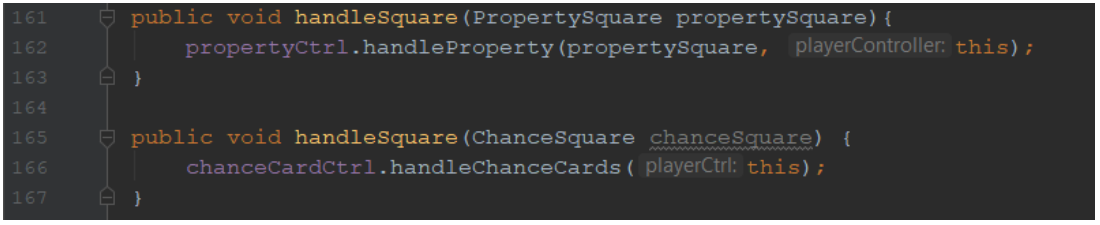
\includegraphics[scale=0.5]{pics/handle_square.png}
        \caption{Kode over handleSquare()}\label{fig:handle_square}
    \end{figure}
        Disse handleSquare metoder bliver kaldt fra landedOn() metoden i felterne, som har en lokal reference til PlayerController (Visitor), som kan ses i Figur~\ref{fig:landed_on} nedenfor. Feltet sender sig selv som et argument ved at bruge “this”. På den måde bliver der valgt og udført den rigtige handleSquare metode i ud fra hvilken type argument der blev sendt. Med andre ord, når der kaldes handleSquare(this), så der udføres den metode, som tager imod den type af felt, der sendes som argument og programmets videre forløb fortsættes i forhold til det. Man kan sige, at det er en anden måde at kontrollere programmets “workflow ”.
        \begin{figure}[H]
            \centering
            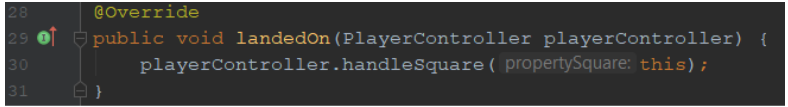
\includegraphics[scale=0.6]{pics/landed_on.PNG}
            \caption{Kode over landedOn()}\label{fig:landed_on}
        \end{figure}


       \paragraph{Bagside \newline}
        Det er dog en bagside ved at bruge Visitor pattern, at der skal tilføjes en ny handleSquare() metode, hver gang der tilføjes en ny felt-type, som kommer til at være som en parameter i denne handleSquare() metode. Det er dog ret usandsynligt, at der kommer flere felter, da felterne i et matador-regelsæt er ret universale.
\end{document}